% Number of images/objects:        25,596\\
% Number of object names:  450\\
% Number of collection nodes (synsets):    52 \\

We take data from \vg~\cite{krishna2016visualgenome}, which
% aims to provide a full set of descriptions of the scenes which images depict in order to spur complete scene understanding. 
contains a dense region-based labeling of $108$K~images with, inter alia, objects, attributes and relationships,  %object descriptions, attributes, and relationships, as well as question-answer pairs, 
all linked to WordNet synsets \cite{fellbaum1998wordnet}.
\vg suits our purpose of collecting names for naturalistic instances of common objects, as it has images of varying complexity, with close-ups as well as images with many objects.
%As common in Computer Vision, O
Objects are localized as 
%identified via
 bounding boxes, as in Figure~\ref{fig:cake}.% 
\footnote{We use image and object interchangeably in the following, since we only selected one target object per image (i.e., each object and image in VG is chosen at most once).}

\subsection{Sampling of Instances}
\label{ssec:sampling}
 % of frequent classes/names in  \vgenome, which, at the same time, have been frequently/commonly studied in the psycholinguistic literature. 
%Criteria: From CV: select images depicting objects with relatively frequent names; From CogSci: select objects which have been frequently studied in cognitive science/psychological norming studies; we chose McRae et al. as basis.
We selected images from seven domains: six based on McRae et al.'s  (\cite{mcrae2005semantic}) feature norms, a dataset widely used in Psycholinguistics that comprises common objects of different categories (e.g.,~\textsc{animals}, \textsc{furniture}), and \textsc{person}, because it is a very frequent category in \vg.
% We start from the concepts of McRae et al.'s feature norms (REF), which are common objects of different categories (e.g.,~\textsc{animals}, \textsc{furniture}) and, as such, have a high overlap with standard datasets of object norming studies (REFS).
% We added the \textsc{person} category because it is very frequent category in \vgenome.

Within each domain, we aimed at collecting instances at different taxonomic levels  to cover a wide range of phenomena, but this is not straightforward because ontological taxonomies do not align well with the lexicon (for instance, \textit{dog} and \textit{cow} are both mammals, but \textit{dog} has many more common subcategories), and most domains are not organized in a clear taxonomy %in the first place 
(e.g.\ \textsc{home}).
% Standard taxonomies do not align well with name variability; for instance, people use more varied names for types of dogs than for types of cows, while both dogs and cows are mammals.
Instead, we defined a set of synsets ($52$\ in total) that we would use to collect our object instances from \vg, balancing variability.
From the set of synsets that match or subsume the concepts in the McRae norms, we kept those with a high number of \vg object instances of different names.
For example, \vg instances subsumed by McRae's \textsl{dog} were named \textsl{beagle, greyhound, puppy, bulldog}, etc., while McRae's \textsl{duck}, \textsl{goose}, or \textsl{gull} did not have name variants in \vg, so we kept \textsl{dog} and \textsl{bird} (which subsumes \textsl{duck}, \textsl{goose}, or \textsl{gull}) as collection synsets.

We then retrieved all VG images depicting an object whose name matches or is subsumed by words in one of these synsets; we refer to these words as \textit{seeds} ($450$\ in total).
We did not consider objects with names in plural form, with parts-of-speech other than nouns\footnote{We obtained tags with CoreNLP \cite{manning2014stanford}.}, or that were multi-word expressions (e.g.,~\textsl{pink bird}). 
We further only considered objects whose bounding box covered~\mbox{$20-90\%$} of the image area.
% We based the definition of our set of nodes on the WN (REF) synsets of the McRae concepts (e.g.,~dog, duck, goose, gull), the nominal WordNet hierarchy, and the frequency distribution of the VG object names' synsets.\footnote{TODO: need to be clear from the general description of VG that the frequ. of instances labeled with the synset of the object name is meant.} 
% First, we selected a set of collection node candidates---synsets which match (e.g.,~\textsl{dog, duck, goose, gull}) or subsume (e.g.,~\textsl{mammal, bird}) the McRae synsets\footnote{Specific synset IDs, e.g.,~dog.n.01, are omitted for readability.}. 
% From these candidates we kept those as collection nodes which had a high frequency of VG object instances of different names. For example, VG instances  subsumed by McRae's \textsl{dog} were named \textsl{beagle, greyhound, puppy, bulldog}, etc., while McRae's \textsl{duck, goose}, or \textsl{gull} did not have name variants in VG, so we kept \textsl{dog} and \textsl{bird} as collection nodes.
%\paragraph{Collection of instance candidates}
% Goal of above procedure was the collection of instances of selected object classes---our nodes--- whose VG names correspond to or subsume (are hypernyms of) a McRae concept, and whose object names differ, that is, of which we can expect that people possess different names for them (e.g.,~\textsl{duck, goose, gull} for \textsl{bird}).
% \paragraph{Sampling of instances}
Because of the Zipfian distribution of names, and to balance the collection, we sampled instances depending on the size of the seeds: up to $500$\ instances for seeds with up to $800$\ objects, and up to $1000$\ instances for larger seeds. %\textbf{double-check}
This yielded a dataset of\ $31,093$~instances, which was further pruned during annotation. 
See Section\ \ref{ssec:elicitation} and the Supplemental Material for details on the pruning. 
% \begin{itemize}
% \item rows: domains (if we go for long paper: then one row per collection node?)
% \item columns:
%   \begin{enumerate}
%   \item \# collection nodes
%   \item collection nodes (list)
%   \item \# unique VG names
%   \item example VG names
%   \item \# unique objects
%   \item \# unique images (? not sure if necessary; maybe only one of unique {objects, images})
%   \end{enumerate}
% \end{itemize}

\subsection{Elicitation Procedure}
\label{ssec:elicitation}
To elicit object names, we set up a crowdsourcing task on Amazon Mechanical Turk (AMT).
In initial pilot studies, we found object identification via bounding boxes to be problematic.
In some cases, the bounding box was not clear; in others, AMT workers named objects that were more salient than the one signaled by the box (for instance, for a box around a jacket, the man wearing it).
We took special care of minimizing this issue in two ways: Specifying the instructions such that workers pay close attention to what object is being indicated in the box, and pruning the set of images via an initial collection round (9 workers per task, i.e.,\ 9 names/object) in which we allowed workers to indicate whether the object was occluded or the box unclear. 
%The Appendix~\ref{app:instructions} contains the task instructions and details about the pruning and data procedure.
We eliminated around $5.5$K\ images based on pruning, obtaining the final dataset with $25,596$\ images. 
(We refer to the Supplemental Material for the task instructions and more details on the pruning and the dataset.) 
We then did 3 more collection rounds, and shuffled the set of images per task between each round. 
Workers could only participate in one round, to avoid workers annotating an instance more than once. 
We obtained a total of 36 names per image (i.e.,\ object).
As will become clear in the analysis, while object identification remains an issue despite these precautions, most mismatches between \vg annotations  and our data cannot be considered mistakes, and the annotation results have significant implications for the study of object naming in L\&V (see discussion in Sections~\ref{sec:analysis} and \ref{sec:modeling}).
Overall $841$\ workers took part in the data elicitation, with a median of  $261$\ instances \mbox{($\textrm{range}=[9,17K]$)} per worker.


\begin{table*}[htp]
	\small
	\centering
	\begin{tabular}{lllll}
			\toprule
			Domain & \multicolumn{4}{c}{Synsets}\\
			\midrule			
			buildings      &  house$_1$ (364) &  bridge$_1$ (297) &  shelter$_1$ (169) &  restaurant$_1$ (58)\\
			&  outbuilding$_1$ (31) &  hotel$_1$ (19) &  housing$_1$ (17) &  place\_of\_worship$_1$ (12)     \\
			people         &  woman$_1$ (1768) &  man$_1$ (1167) &  male\_child$_1$ (853) &  athlete$_1$ (396) \\
			&  child$_1$ (333) &  creator$_2$ (11) &  professional$_1$ (5)    \\
			home           &  furnishing$_2$ (5355) &  vessel$_3$ (525) &  kitchen\_utensil$_1$ (132) &  crockery$_1$ (92) \\
			&  cutlery$_2$ (82) &  tool$_1$ (72) &  lamp$_1$ (34)    \\
			clothing       &  shirt$_1$ (968) &  overgarment$_1$ (786) &  dress$_1$ (199) &  headdress$_1$ (135)\\
			 &  neckwear$_1$ (65) 		&  robe$_1$ (27) &  glove$_2$ (7) &  footwear$_1$ (5)    \\
			vehicles       &  aircraft$_1$ (1208) &  train$_1$ (957) &  car$_1$ (727) &  motorcycle$_1$ (564) \\
			&  truck$_1$ (559) &  boat$_1$ (499) &  ship$_1$ (38)    \\
			food           &  dish$_2$ (812) &  baked\_goods$_1$ (770) &  foodstuff$_2$ (280) &  vegetable$_1$ (48) \\
			&  edible\_fruit$_1$ (42) 	&  beverage$_1$ (23)   \\
			animals\_plants &  ungulate$_1$ (2037) &  horse$_1$ (833) &  feline$_1$ (763) &  dog$_1$ (688) \\
			&  bird$_1$ (389) &  flower$_1$ (44) &  rodent$_1$ (27) &  insect$_1$ (12) \\ 
			&  fish$_1$ (11) &   \\
			\bottomrule
		\end{tabular}
		\caption{Overview of our dataset: Synset nodes for each domain (subscript indicates synset number; number of instances in parentheses). %\textbf{double-check}
			\label{tab:overview_dataset2}}
	\end{table*}
%
%
\begin{table*}[htp]
	\small
	\centering
	\begin{tabular}{@{~}l@{~}l@{~}l@{~}l@{~}l@{~}l@{~}l}
		\toprule
		vehicles &            food & animals\_plants &           home &        buildings &             people &      clothing \\
		\midrule
		train (954) &  pizza (518) &  giraffe (915) &  bed (888) &  house (340) &  boy (853) &  shirt (904) \\
		car (642) &  cake (261) &  horse (822) &  bench (714) &  bridge (274) &  man (806) &  jacket (451) \\
		plane (485) &  bread (186) &  cat (754) &  table (687) &  dugout (91) &  woman (766) &  coat (267) \\
		airplane (479) &  sandwich (153) &  dog (654) &  desk (672) &  tent (53) &  girl (650) &  dress (190) \\
		motorcycle (466) &  bun (143) &  zebra (461) &  counter (516) &  restaurant (33) &  lady (342) &  hat (77) \\
		truck (465) &  cheese (110) &  cow (324) &  couch (366) &  overpass (23) &  guy (330) &  t-shirt (62) \\
		boat (450) &  donut (78) &  bird (295) &  chair (365) &  grill (22) &  child (230) &  tie (51) \\
		jet (106) &  salad (70) &  sheep (216) &  carpet (307) &  garage (18) &  batter (110) &  blazer (43) \\
		aircraft (85) &  sauce (68) &  bull (48) &  bowl (219) &  hotel (16) &  kid (85) &  hood (26) \\
		van (76) &  apple (33) &  flower (40) &  curtain (182) &  castle (14) &  skateboarder (80) &  cap (20) \\
		\bottomrule
	\end{tabular}
	\caption{Overview of our ManyNames dataset: Top-10 VG names for each domain (number of instances in parentheses). %\textbf{double-check}
		\label{tab:overview_dataset1}}
\end{table*}

Figures~\ref{fig:instructions1} and \ref{fig:instructions2} contain the instructions for our subjects in the first round and rounds 2-4, respectively.
After the first round, based on the opt-out annotation, we kept images that met all the following conditions (thresholds were estimated via manual inspection):
\begin{itemize}
\item they were not marked as occluded by any subject;
\item ``Bounding box is unclear'' was marked at most twice;
\item at most 17\% of elicited names were in plural form (to remove cases where the bounding box contains several objects);
\item the most frequent elicited name is of the same domain as the \vgenome name.
\end{itemize}
This yielded $25,596$ images, discarding $5,497$.

\begin{figure*}[htp]
  \centering
  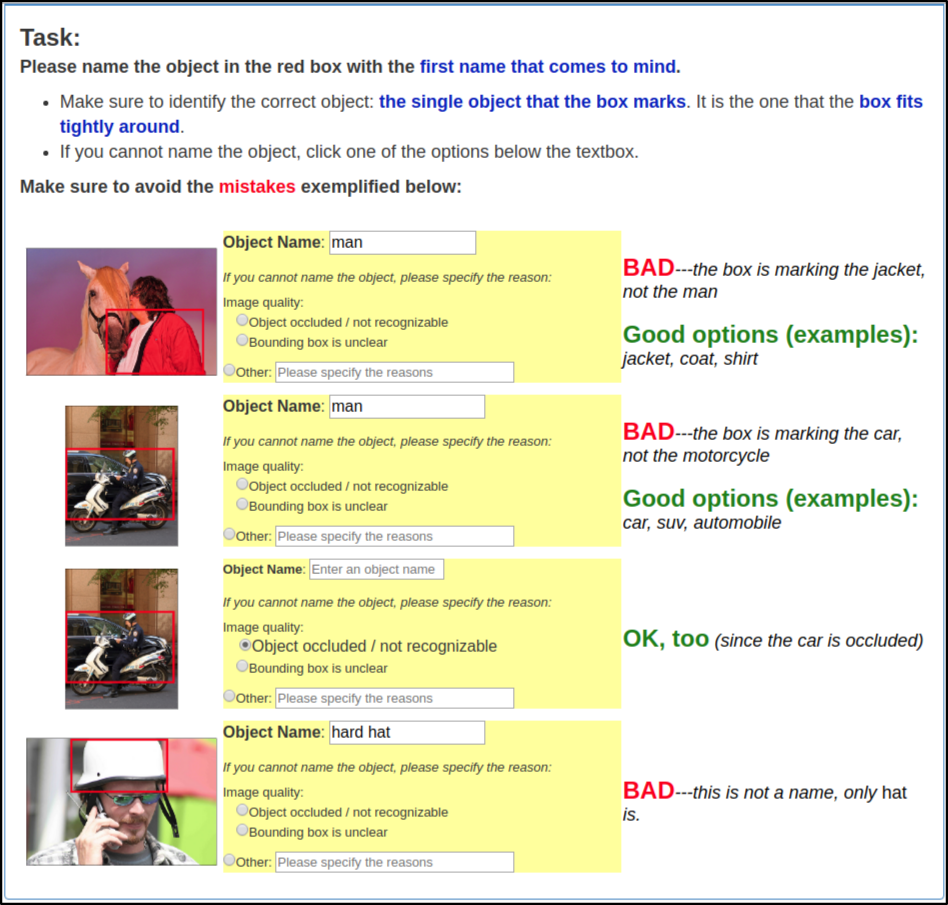
\includegraphics[width=1.5\columnwidth]{figures/round0.png}
  \caption{Instructions for AMT annotators for the first round.}
  \label{fig:instructions1}
\end{figure*}

\begin{figure*}[htp]
  \centering
  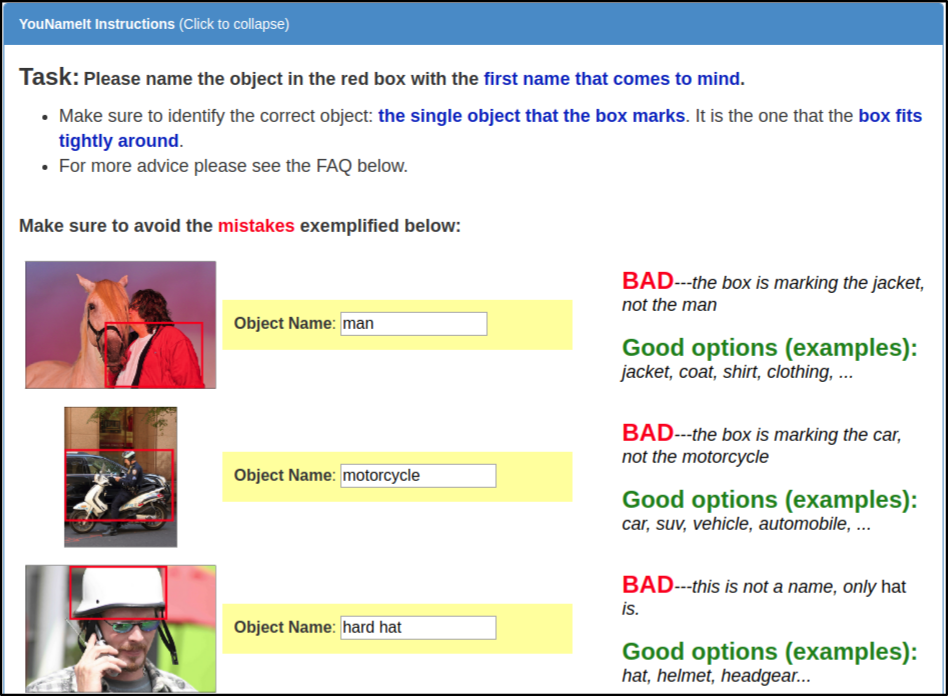
\includegraphics[width=1.5\columnwidth]{figures/round1+_p1.png}
  \caption{Instructions for AMT annotators for rounds~$2$ to~$4$. They were accompanied by the FAQ in Figure~\ref{fig:faq}}
  \label{fig:instructions2}
\end{figure*}
%
\begin{figure*}[htp]
  \centering
  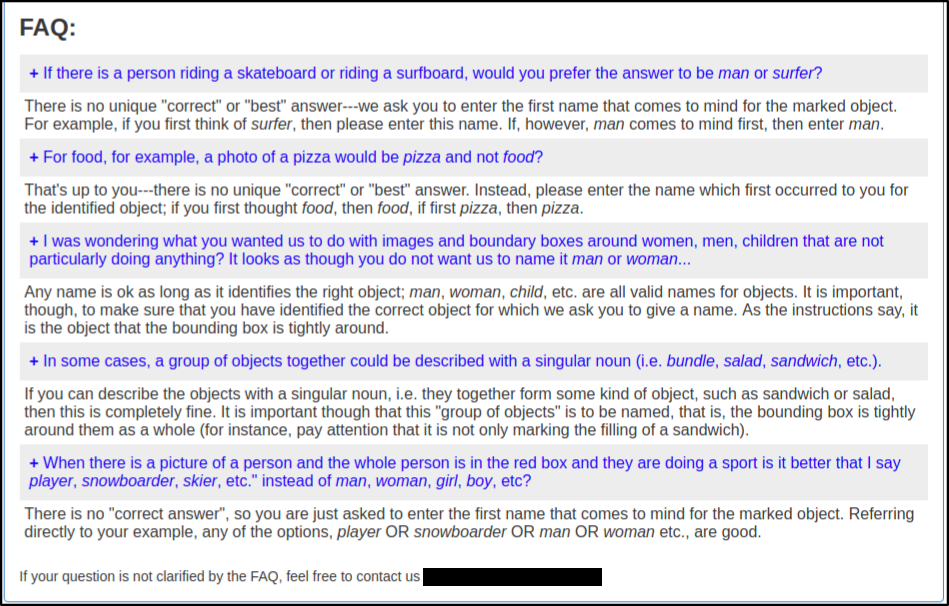
\includegraphics[width=1.5\columnwidth]{figures/round1+_p2.png}
  \caption{FAQ accompanying the instructions for AMT annotators for rounds~$2$ to~$4$.}
  \label{fig:faq}
\end{figure*}

%\cs{Maybe say something about the rejections, if space permits it.}


%%% Local Variables:
%%% mode: latex
%%% TeX-master: "lrec2020naming"
%%% End:


